%% LyX 2.2.3 created this file.  For more info, see http://www.lyx.org/.
%% Do not edit unless you really know what you are doing.
\documentclass[12pt,english]{article}
\usepackage[osf]{mathpazo}
\renewcommand{\sfdefault}{lmss}
\renewcommand{\ttdefault}{lmtt}
\usepackage[T1]{fontenc}
\usepackage[latin9]{inputenc}
\usepackage[paperwidth=30cm,paperheight=35cm]{geometry}
\geometry{verbose,tmargin=3cm,bmargin=3cm}
\setlength{\parindent}{0bp}
\usepackage{amsmath}
\usepackage{amssymb}

\makeatletter

%%%%%%%%%%%%%%%%%%%%%%%%%%%%%% LyX specific LaTeX commands.
%% Because html converters don't know tabularnewline
\providecommand{\tabularnewline}{\\}

%%%%%%%%%%%%%%%%%%%%%%%%%%%%%% User specified LaTeX commands.
\usepackage{tikz}
\usetikzlibrary{matrix,arrows,decorations.pathmorphing}
\usetikzlibrary{shapes.geometric}
\usepackage{tikz-cd}
\usepackage{amsthm}
\theoremstyle{plain}
\newtheorem{theorem}{Theorem}[section]
\newtheorem{lemma}[theorem]{Lemma}
\newtheorem{prop}{Proposition}[section]
\newtheorem*{cor}{Corollary}
\theoremstyle{definition}
\newtheorem{defn}{Definition}[section]
\newtheorem{ex}{Exercise} 
\newtheorem{example}{Example}[section]
\theoremstyle{remark}
\newtheorem*{rem}{Remark}
\newtheorem*{note}{Note}
\newtheorem{case}{Case}
\usepackage{graphicx}
\usepackage{amssymb}
\usepackage{tikz-cd}
\usetikzlibrary{calc,arrows,decorations.pathreplacing}
\tikzset{mydot/.style={circle,fill,inner sep=1.5pt},
commutative diagrams/.cd,
  arrow style=tikz,
  diagrams={>=latex},
}

\usepackage{babel}
\usepackage{hyperref}
\hypersetup{
    colorlinks,
    citecolor=black,
    filecolor=black,
    linkcolor=black,
    urlcolor=black
}
\usepackage{pgfplots}
\usetikzlibrary{decorations.markings}
\pgfplotsset{compat=1.9}

\makeatother

\usepackage{babel}
\begin{document}

\title{An Interesting Complex and its Homology}

\author{Michael Nelson}

\maketitle
\pagebreak{}

\tableofcontents{}

\pagebreak{}

\section{Notations and Preliminary Material}

\subsection{Homological Algebra}

~~~Throughout this article, $R$ be a ring and let $K$ be a field
of characteristic $2$. Recall that a \textbf{chain complex} $A=(A_{\bullet},d_{\bullet})$
\textbf{over} $R$ is a sequence of $R$-modules $A_{i}$ and morphisms
$d_{i}:A_{i}\to A_{i-1}$ \begin{equation}\label{diagramA}\begin{tikzcd} A := \cdots \arrow[r] & A_{i+1} \arrow[r,"d _{i+1}"] & A_i  \arrow[r," d _i "] & A_{i-1} \arrow[r] & \cdots \end{tikzcd}\end{equation}

such that $d_{i}\circ d_{i+1}=0$ for all $i\in\mathbb{Z}$. The condition
$d_{i}\circ d_{i+1}=0$ is equivalent to the condition $\text{Ker}(d_{i})\supset\text{Im}(d_{i+1})$.
With this in mind, we define the \textbf{$i$th} \textbf{homology
of the chain complex} to be 
\[
H_{i}(A):=\text{Ker}(d_{i})/\text{Im}(d_{i+1}).
\]
A \textbf{chain map} between two chain complexes $(A_{\bullet},d_{\bullet})$
and $(A'_{\bullet},d'_{\bullet})$ over $R$ is a sequence $\varphi_{\bullet}$
of $R$-module homomorphisms $\varphi_{i}:A_{i}\to B_{i}$ such that
$d_{i}\varphi_{i-1}=\varphi_{i}d_{i-1}'$ for all $i$. It then follows
that a chain map gives rise to map an induced map on homology $H_{i}(A)\to H_{i}(A')$. 

~~~The dual notion to a chain complex is a \textbf{cochain complex
}$A=(A^{\bullet},d^{\bullet})$ over $R$. It is just a chain complex,
except we label things differently. Namely, we replace subscripts
with superscripts. We will be studying objects which have compatible
chain and cochain complex structures.

~~~~~~To simplify notation, we think of $R$ as a trivially
graded ring, that is, the degree equals $0$ part is $R$ and all
the other homogeneous components are $0$. We think of the complex
(\ref{diagramA}) as a graded $R$-module $A$ (where the degree $i$
homogoneous component is $A_{i}$) together with an endomorphism $d$
of degree $-1$ such that $d^{2}=0$. We write $A[j]$ for the graded
module obtained from $A$ by the rule $A[j]_{i}=A_{i+j}$. 

\subsection{Gr�bner Basis}

~~~Throughout this article, let $S=K[x_{1},\dots,x_{n}]$, $I$
be a homogeneous ideal in the polynomial ring $K[x_{1},\dots,x_{n}]$,
and let $G=\{g_{1},g_{2}\dots,g_{r}\}$ be the reduced gr�bner basis
for $I$ with respect to a fixed monomial ordering (see the book ``Ideals,
Varieties, and Algorithms: An Introduciton to Computation Algebraic
Geometry and Commutative Algebra'' for details). Recall that $f\in K[x_{1},\dots,x_{n}]$
can be written in the form $f=g+r$, where $g\in I$ and no term of
$r$ is divisible by any element of $\text{LT}(I),$ and, moreover,
$g$ and $r$ are uniquely determined. We use the notation $f^{G}:=r$
and call this the \textbf{normal form of} $f$ \textbf{with respect
to $I$ }(or simply the \textbf{normal form of $f$ }if the there
is no confusion of the ideal $I$). It follows from uniqueness of
$f^{G}$ and $f-f^{G}$ that taking the normal form of a polynomial
is a $K$-linear map:
\begin{equation}
\alpha f_{1}^{G}+\alpha_{1}f_{2}^{G}=(\alpha_{1}f_{1}+\alpha_{2}f_{2})^{G}\qquad\text{for all }\alpha_{1},\alpha_{2}\in K\text{ and }f_{1},f_{2}\in S.\label{eq:Klinearity}
\end{equation}

~~~Recall that $S$ is a graded $K$-algebra, where the homogeneous
component $S_{i}$ is the $K$-vector space of all homogeneous polynomials
$f\in S$ of degree $i$. Since $I$ is a homogeneous ideal, the ring
$S/I$ also inherits the structure of a graded algebra over $K$,
where the homogeneous component $(S/I)_{i}$ is $(S/I)_{i}:=S_{i}/(I\cap S_{i})$.
In fact, $S/I$ is isomorphic as a graded $K$-vector space to $S_{I}:=\text{Span}_{K}(x^{\alpha}\mid x^{\alpha}\notin\langle\text{LT}(I)\rangle)$,
where $S_{I}$ has homogeneous components $(S_{I})_{i}=\text{Span}_{K}(x^{\alpha}\mid x^{\alpha}\notin\langle\text{LT}(I)\rangle\text{ and \text{deg}}(x^{\alpha})=i\rangle$.
The isomorphism is given by mapping $\overline{f}\in(S/I)_{i}$ to
$f^{G}\in(S_{I})_{i}$, where $K$-linearity follows from (\ref{eq:Klinearity}).
The inverse of this map is given by mapping $f\in(S_{I})_{i}$ to
$\overline{f}\in(S/I)_{i}$. Composing this map with the natural inclusion
map $(S_{I})_{i}\subset S_{i}$, we obtain an injective map $(S/I)_{i}\to S_{i}$,
call this map $\varphi$. 

~~~Similarly, $I$ has a graded $K$-module structure, where the
homogeneous component $I_{i}$ is $I_{i}:=I\cap S_{i}$, and the map
from $S_{i}$ to $I_{i}$ sending $f$ to $f-f^{G}$ is $K$-linear
(since we are working over a characteristic $2$ field, we can just
write $f+f^{G}$). Call this map $\psi$. Since $f^{G}=0$ if and
only if $f\in I$, the natural inclusion map $I_{i}\subset S_{i}$
splits $\psi$. Combining everything together, we obtain the following
short exact sequences of $K$-vector spaces:

\begin{equation}\label{diagram1}\begin{tikzcd}[column sep=huge, row sep=0.4] 0 \arrow[r] & (S/I)_i \arrow[r, "\varphi "] & S_i \arrow[r, "\psi "] & I_i \arrow[r] & 0 \\ & \overline{f} \arrow[r,mapsto,shorten >=0.2cm,shorten <=0.2cm] & f^G \\ && f \arrow[r,mapsto,shorten >=0.2cm,shorten <=0.2cm] & f + f^G \end{tikzcd}\end{equation}

\begin{example}\label{example} Consider $S=K[x,y]$ and $I=\langle xy+y^{2},x^{3}\rangle$.
We first use Singular to compute a Gr�bner basis of $G$ of $I$ with
respect to graded reverse lex order. We obtain $G=\{g_{1},g_{2},g_{3}\}$.
where $g_{1}=xy+y^{2}$, $g_{2}=x^{3}$, and $g_{3}=y^{4}$. Then
\begin{align*}
I_{0} & =0 & (S/I)_{0} & =K\cdot\overline{1} & (S_{I})_{0} & =K\\
I_{1} & =0 & (S/I)_{1} & =K\overline{x}+K\overline{y} & (S_{I})_{1} & =Kx+Ky\\
I_{2} & =Kg_{1} & (S/I)_{2} & =K\overline{x}^{2}+K\overline{y}^{2} & (S_{I})_{2} & =Kx^{2}+Ky^{2}\\
I_{3} & =Kxg_{1}+Kyg_{1}+Kg_{2} & (S/I)_{3} & =K\overline{y}^{3} & (S_{I})_{3} & =Ky^{3}\\
I_{4} & =S_{4} & (S/I)_{4} & =0 & (S_{I})_{4} & =0\\
 & \vdots &  & \vdots &  & \vdots
\end{align*}

\end{example}

\section{$\mathbf{A}(I),$ $\mathbf{A}(S)$, and $\mathbf{\mathbf{A}}(S/I)$}

\subsection{Construction of $\mathbf{A}_{\bullet}(S)$}

~~~Let $d_{i}:S_{i}\to S_{i-1}$ be the map given by $d_{i}:=\sum_{j=1}^{n}\partial_{x_{j}}$.
This map is clearly $K$-linear, and since we are working over a field
of characteristic $2$, we have $d^{2}=0$: Let $x_{1}^{\alpha_{1}}\cdots x_{n}^{\alpha_{n}}$
be a monomial in $S_{i}$, then
\begin{align*}
d^{2}\left(x_{1}^{\alpha_{1}}\cdots x_{n}^{\alpha_{n}}\right) & =\left(\sum_{k=1}^{n}\partial_{x_{k}}\right)^{2}\left(x_{1}^{\alpha_{1}}\cdots x_{n}^{\alpha_{n}}\right)\\
 & =\left(\sum_{k=1}^{n}\partial_{x_{k}}^{2}\right)\left(x_{1}^{\alpha_{1}}\cdots x_{n}^{\alpha_{n}}\right)\\
 & =\sum_{k=1}^{\infty}\alpha_{k}(\alpha_{k}-1)x_{1}^{\alpha_{k}-2}\\
 & =0.
\end{align*}

Thus, $d$ gives the graded $K$-algebra $S$ the structure of a chain
complex over $K$, which we call $\mathbf{A}_{\bullet}(S):=(S_{\bullet},d_{\bullet})$. 

\subsection{Construction of $\mathbf{A}_{\bullet}(S/I)$ }

~~~Since we are working over a field of characteristic $2$. We
describe $d$ in a simpler manner: Let $m=x_{1}^{\alpha_{1}}\cdots x_{n}^{\alpha_{n}}$
be a monomial of degree $i$ in $S$. We can decompose $m$ as $m=uv$,
where 
\[
u=\prod_{\substack{1\leq j\leq n\\
\alpha_{j}\text{ is odd}
}
}x_{j}^{\alpha_{j}}\qquad\text{and}\qquad v=\prod_{\substack{1\leq\ell\leq n\\
\alpha_{\ell}\text{ is even}
}
}x_{\ell}^{\alpha_{\ell}}.
\]
We denote $[m]_{o}=\{1\leq j\leq n\mid\alpha_{j}\text{ is odd}\}$
and $[m]_{e}=\{1\leq\ell\leq n\mid\alpha_{\ell}\text{ is even}\}$.
From this decomposition and the definition of $d_{i}$, we can describe
$d_{i}$ another way: 
\[
d_{i}(m)=\sum_{x_{j}\mid u}x_{j}^{-1}m.
\]
This makes it clear, for example, that $d_{i}$ restricts to a map
$d_{i}:(S_{I})_{i}\to(S_{I})_{i-1}$: If $m$ is not in $\text{LT}(I)$,
then every term $x_{\lambda}^{-1}m$ of $d(m)$ is not in $\text{LT}(I)$
either. Thus, using the isomorphism $(S/I)_{i}\to(S_{I})_{i}$, we
can construct a map $\underline{d}_{i}:(S/I)_{i}\to(S/I)_{i-1}$,
given by $\underline{d}_{i}(\overline{f})=\overline{d_{i}(f^{G})}$
for all $\overline{f}\in(S/I)_{i}$. It's easy to see now that the
map $\underline{d}$ gives the graded $K$-algebra $S/I$ the structure
of a chain complex over $K$, which we call $\mathbf{A}_{\bullet}(S/I):=((S/I)_{\bullet},\underline{d}_{\bullet})$. 

\subsection{Construction of $\mathbf{A}_{\bullet}(S_{I})$}

~~~Recall that $S/I$ is isomorphic as a graded $K$-vector space
to $S_{I}$. In fact, even more is true. We can carry multiplication
from $S/I$ over to $S_{I}$ to make $S_{I}$ into a graded $K$-algebra:
For $f_{1},f_{2}\in S_{I}$, we define multiplication as
\[
f_{1}\cdot f_{2}=(f_{1}f_{2})^{G}
\]

It's easy to see that this is bilinear and that this makes $S_{I}$
isomorphic to $S/I$ as graded $K$-algebras. As seen above, the differential
$d$ restricts to $S_{I}$ and gives the graded $K$-algebra $S_{I}$
the structure of a chain complex over $K$, which we call $\mathbf{A}_{\bullet}(S_{I}):=((S_{I})_{\bullet},d_{\bullet})$.
Clearly we have $\mathbf{A}_{\bullet}(S_{I})\cong\mathbf{A}_{\bullet}(S/I)$,
but it will be useful to swap back and forth between the two of them. 

\subsection{Construction of $\mathbf{A}_{\bullet}(I)$}

~~~Our final construction involves the graded $K$-module $I$.
Using the fact that the inclusion map $I_{i}\subset S_{i}$ splits
$\psi$, we can construct a map $\overline{d}_{i}:I_{i}\to I_{i-1}$,
where $\overline{d}_{i}(f)=d_{i}(f)+d_{i}(f)^{G}$ for all $f\in I_{i}$.
The map $\overline{d}$ gives the graded $K$-module $I$ the structure
of a chain complex over $K$, which we call $\mathbf{A}_{\bullet}(I):=((I)_{\bullet},\overline{d}_{\bullet})$. 

\subsection{Summary and Example}

~~~Summarizing everything up. We have the following chain complexes
over $K$:
\begin{center}
\begin{tabular}{c|c|c}
Chain Complex & Homogeneous Components & Differential\tabularnewline
\hline 
\hline 
$\mathbf{A}_{\bullet}(S):=(S_{\bullet},d_{\bullet})$ & $\mathbf{\mathbf{A}_{\bullet}}(S)_{i}:=S_{i}$  & $d_{i}:S_{i}\to S_{i-1}$\tabularnewline
\hline 
$\mathbf{A}_{\bullet}(I):=((I)_{\bullet},\overline{d}_{\bullet})$ & $\mathbf{A}_{\bullet}(I)_{i}:=I_{i}$ & $\overline{d}_{i}:I_{i}\to I_{i-1}$\tabularnewline
\hline 
$\mathbf{A}_{\bullet}(S/I):=((S/I)_{\bullet},\underline{d}_{\bullet})$ & $\mathbf{A}_{\bullet}(S/I)_{i}:=(S/I)_{i}$ & $\underline{d}_{i}:(S/I)_{i}\to(S/I)_{i-1}$\tabularnewline
\hline 
$\mathbf{A}_{\bullet}(S_{I}):=((S/I)_{\bullet},d_{\bullet})$ & $\mathbf{A}_{\bullet}(S_{I})_{i}:=(S_{I})_{i}$ & $d_{i}:(S_{I})_{i}\to(S_{I})_{i-1}$\tabularnewline
\end{tabular}
\par\end{center}

We now bring these ideas together in the following example.

\begin{example}\label{example} Consider the case where $S=\mathbb{F}_{2}[x,y,z]$
and $I=\langle xy,x^{3},y^{2}z,xz^{3},z^{4},y^{5}\rangle$, where
$G=\{xy,x^{3},y^{2}z,xz^{3},z^{4},y^{5}\}$ is the minimal basis for
$I$. Let's write down the first fiew graded pieces of $\mathbf{A}_{\bullet}(S/I)$:
\begin{align*}
\mathbf{A}_{\bullet}(S/I)_{0} & =\mathbb{F}_{2}\\
\mathbf{A}_{\bullet}(S/I)_{1} & =\mathbb{F}_{2}\overline{x}+\mathbb{F}_{2}\overline{y}+\mathbb{F}_{2}\overline{z}\\
\mathbf{A}_{\bullet}(S/I)_{2} & =\mathbb{F}_{2}\overline{x}^{2}+\mathbb{F}_{2}\overline{x}\overline{z}+\mathbb{F}_{2}\overline{y}^{2}+\mathbb{F}_{2}\overline{y}\overline{z}+\mathbb{F}_{2}\overline{z}^{2}\\
\mathbf{A}_{\bullet}(S/I)_{3} & =\mathbb{F}_{2}\overline{x}^{2}\overline{z}+\mathbb{F}_{2}\overline{x}\overline{z}^{2}+\mathbb{F}_{2}\overline{y}^{3}+\mathbb{F}_{2}\overline{y}\overline{z}^{2}+\mathbb{F}_{2}\overline{z}^{3}\\
\mathbf{A}_{\bullet}(S/I)_{4} & =\mathbb{F}_{2}\overline{x}^{2}\overline{z}^{2}+\mathbb{F}_{2}\overline{y}^{4}+\mathbb{F}_{2}\overline{y}\overline{z}^{3}\\
\mathbf{A}_{\bullet}(S/I)_{5} & =0\\
 & \vdots
\end{align*}

The homology of this chain complex is not trivial. For instance, we
will see that $H_{1}(\mathbf{A}_{\bullet}(S\backslash I))=\mathbb{F}_{2}\overline{d(xy)}$.
Now let's write down the first few graded pieces of $\mathbf{A}_{\bullet}(I)$:
\begin{align*}
\mathbf{A}_{\bullet}(I)_{1} & =0\\
\mathbf{A}_{\bullet}(I)_{2} & =\mathbb{F}_{2}xy\\
\mathbf{A}_{\bullet}(I)_{3} & =\mathbb{F}_{2}x^{3}+\mathbb{F}_{2}x^{2}y+\mathbb{F}_{2}xy^{2}+\mathbb{F}_{2}xyz+\mathbb{F}_{2}y^{2}z\\
 & \vdots
\end{align*}

\end{example}

\section{Differential Graded Algebras}

\subsection{Differential Graded Algebra Structure on $\mathbf{A}_{\bullet}(S)$}

~~~It turns out that $\mathbf{A}_{\bullet}(S)$ is more than just
a chain complex over $K$, in fact it also has the structure of a
differential graded algebra over $\mathbb{F}_{2}$. Before we discuss
this, let's define what a differential graded algebra over a ring
is.

\begin{defn}\label{defn} A \textbf{differential graded algebra over
$R$ }is a chain complex $A=(A_{\bullet},d_{\bullet})$ over $R$
together with $R$-bilinear maps $A_{i}\times A_{j}\to A_{i+j}$,
denoted $(a,b)\mapsto ab$, such that the \textbf{Leibniz law }holds:
\begin{equation}
d_{i+j}(ab)=d_{i}(a)b+(-1)^{i}ad_{j}(b).\label{eq:leibnizlaw}
\end{equation}
for all $a,b\in A$. 

\end{defn}

\begin{rem}\label{rem} To ease notation, we usually drop the subscripts
in (\ref{eq:leibnizlaw}) as long as everything is clear. Combining
this with the fact that we are working over a field of characteristic
$2$, we can simplify (\ref{eq:leibnizlaw}) to 
\begin{equation}
d(ab)=d(a)b+ad(b).\label{eq:leibniz2}
\end{equation}

\end{rem}

~~~Since $S$ is already a graded $K$-algebra, we already have
bilinear maps $S_{i}\times S_{j}\to S_{i+j}$. Also, the Leibniz law
(\label{eq:leibnizlaw}) follows since $d$ is defined in terms of
partial derivatives. 

\subsection{Almost Differential Graded Algebra Structure on $\mathbf{A}_{\bullet}(S_{I})$.}

~~~It is not necessarily the case that $\mathbf{A}_{\bullet}(S_{I})$
is a differential graded algebra over $K$. For instance, consider
$I=\langle x^{5}\rangle$ in $\mathbb{F}_{2}[x]$. Then $d(x\cdot x^{5})=d((x^{6})^{G})=0$,
but $d(x)\cdot x^{4}+x\cdot d(x^{4})=(x^{4})^{G}=x^{4}$. On the other
hand, if we make an assumption on the reduced Gr�bner basis $G=\{g_{1},g_{2}\dots,g_{r}\}$,
then we do get a differential graded algebra:

\begin{prop}\label{propdgalgebrasi} Suppose $d(g_{i})=0$ for all
$1\leq i\leq r$. Then 
\[
d(f^{G})=d(f)^{G}
\]
for all $f\in S$. In particular, $\mathbf{A}_{\bullet}(S_{I})$ is
a differential graded algebra over $K$. \end{prop}

\begin{proof} From the division algorithm, we have $f=g_{1}h_{1}+\cdots+g_{r}h_{r}+f^{G}$
for some $h_{1},\dots,h_{r}\in S$. Thus 
\begin{align*}
d(f) & =d(g_{1}h_{1}+\cdots+g_{r}h_{r}+f^{G})\\
 & =g_{1}d(h_{1})+\cdots+g_{r}d(h_{r})+d(f^{G}).
\end{align*}
Since $g_{1}d(h_{1})+\cdots+g_{r}d(h_{r})\in I$ and no term of $d(f^{G})$
is divisible by any element of $\text{LT}(I)$, it follows from uniqueness
of the remainder that $d(f^{G})=d(f)^{G}$. 

~~~Now we show that this implies $\mathbf{A}_{\bullet}(S_{I})$
is a differential graded algebra over $K$. Let $f_{1},f_{2}\in S_{I}$.
Then 
\begin{align*}
d(f_{1}\cdot f_{2}) & =d((f_{1}f_{2})^{G})\\
 & =(d(f_{1}f_{2}))^{G}\\
 & =(d(f_{1})f_{2}+f_{1}d(f_{2}))^{G}\\
 & =(d(f_{1})f_{2})^{G}+(f_{1}d(f_{2}))^{G}\\
 & =d(f_{1})\cdot f_{2}+f_{1}\cdot d(f_{2}).
\end{align*}

\end{proof}

\begin{example}\label{example} Consider $S=K[x,y]$ and $I=\langle xy^{2}+y^{3},x^{3}+x^{2}y\rangle$.
Then $G=\{xy^{2}+y^{3},x^{3}+x^{2}y\}$ is the reduced Gr�bner basis
with respect to degree lexicographical monomial order. Thus $\text{LT}(I)=\langle xy^{2},x^{3}\rangle$.
Let's get acquainted with $S_{I}$. First, let's write the first few
homogeneous terms of $S_{I}$:
\begin{align*}
(S_{I})_{0} & =K\\
(S_{I})_{1} & =Kx+Ky\\
(S_{I})_{2} & =Kx^{2}+Kxy+Ky^{2}\\
(S_{I})_{3} & =Kx^{2}y+Ky^{3}\\
(S_{I})_{4} & =Ky^{4}\\
(S_{I})_{5} & =Ky^{5}\\
 & \vdots
\end{align*}

Next, we multiply some elements together in $S_{I}$ in the multiplication
table below
\begin{center}
\begin{tabular}{c|ccc}
$\cdot$ & $x$ & $y$ & $y^{3}$\tabularnewline
\hline 
$x^{2}y$ & $y^{4}$ & $y^{4}$ & $y^{6}$\tabularnewline
$x^{2}$ & $x^{2}y$ & $x^{2}y$ & $y^{5}$\tabularnewline
$x$ & $x^{2}$ & $xy$ & $y^{4}$\tabularnewline
\end{tabular}
\par\end{center}

Now observe that $d(xy^{2}+y^{3})=d(x^{3}+x^{2}y)=0$. Thus, by Proposition~(\ref{propdgalgebrasi}),
$\mathbf{A}_{\bullet}(S_{I})$ is a differential graded algebra.\end{example}

\section{Calculating the Homologies $H_{i}(\mathbf{A}_{\bullet}(I))$, $H_{i}(\mathbf{A}_{\bullet}(S))$,
and $H_{i}(\mathbf{A}_{\bullet}(S/I))$}

We first start with what is essentially a consequence of $\mathbf{A}_{\bullet}(S)$
being a differential graded algebra. 

\begin{prop}\label{prop} $H_{i}(\mathbf{A}(S))=0$ for all $i\geq0$.
\end{prop}

\begin{proof} Let $f$ be a homogeneous polynomial of degree $i$
such that $d(f)=0$. Then for any $x_{\lambda}\in S_{1}$, we have
\[
d(x_{\lambda}f)=d(x_{\lambda})f+x_{\lambda}d(f)=f.
\]
Therefore, $\text{Ker}(d)=\text{Im}(d)$, which proves the claim.
\end{proof}

\begin{prop}\label{proplongexact} The differential $d$ induces isomorphisms
$H_{i}(\mathbf{A}_{\bullet}(I))\cong H_{i-1}(\mathbf{A}_{\bullet}(S/I))$
for all $i>0$. \end{prop}

\begin{proof} The short exact sequence (\ref{diagram1}) gives rise
to a long exact sequence of chain complexes over $K$:

\begin{center}\begin{tikzcd} 0 \arrow[r] & \mathbf{A}(S / I) \arrow[r] & \mathbf{A}(S) \arrow[r] & \mathbf{A}(I) \arrow[r] & 0. \end{tikzcd}\end{center}

From this short exact sequence of chain complexes over $K$, we obtain,
for all $i>0$, the exact sequences

\begin{center}\begin{tikzcd} 0 = H_i ( \mathbf{A}(S) ) \arrow[r] & H_i ( \mathbf{A}(I) ) \arrow[r, "d " ] & H_{i-1} ( \mathbf{A}(S / I)) \arrow[r] &  H_{i-1} ( \mathbf{A}(S) ) = 0, \end{tikzcd}\end{center}where
$d$ is obtained by working out the details of the connecting map.
\end{proof}

\begin{prop}\label{prop} Let $m$ be a monomial such that $x_{\mu}m\in I$
for all $\mu\in[m]_{e}$. Fix $\mu_{0}\in[m]_{e}$. If $x_{\lambda}^{-1}x_{\mu_{0}}m\notin I$
for every $\lambda\in[x_{\mu_{0}}m]_{o}$, then $\overline{d(x_{\mu_{0}}m)}$
represents a nontrivial element in $H(\mathbf{A}_{\bullet}(S/I))$.
\end{prop}

\begin{proof} Saying $x_{\lambda}^{-1}x_{\mu_{0}}m\notin I$ for
every $\lambda\in[x_{\mu_{0}}m]_{o}$, is equivalent to saying $d(x_{\mu_{0}}m)^{G}=d(x_{\mu_{0}}m)$.
Thus, 
\begin{align*}
\underline{d}(\overline{d(x_{\mu_{0}}m)}) & =d(d(x_{\mu_{0}}m)^{G})\\
 & =d(d(x_{\mu_{0}}m))\\
 & =0
\end{align*}
implies $\overline{d(x_{\mu_{0}}m)}$ represents an element in $H(\mathbf{A}_{\bullet}(S/I))$.
To see that this element is nontrivial, note that the condition $x_{\mu}m\in I$
for all $\mu\in[m]_{e}$ implies $\overline{m}\notin\text{Im}(\underline{d})$.
Since $\overline{m}$ is a term in $\overline{d(x_{\mu_{0}}m)}$,
this implies $\overline{d(x_{\mu_{0}}m)}\notin\text{Im}(d)$ either.

\end{proof}

\section{Duality}

~~~For a $K$-vector space $V$, let $V^{\star}:=\text{Hom}_{K}(V,K)$.
Then $(S/I)^{\star}:=\text{Hom}_{K}(S/I,K)$, $S^{\star}:=\text{Hom}_{K}(S,K)$,
and $I^{\star}:=\text{Hom}_{K}(I,K)$ are all graded $K$-modules,
where the homogeneous components are $(S/I)_{i}^{\star},$ $S_{i}^{\star}$,
and $I_{i}^{\star}$ respectively. To get an isomorphism from $S_{i}$
to $S_{i}^{\star}$, we map the monomial $x^{\alpha}\in S_{i}$ to
the element $\varphi_{x^{\alpha}}\in S_{i}^{\star}$, where 
\[
\varphi_{x^{\alpha}}(x^{\beta})=\begin{cases}
0 & \text{if }\alpha\neq\beta\\
1 & \text{if }\alpha=\beta
\end{cases}
\]
for all monomials $x^{\beta}\in S_{i}$. The isomorphisms $(S/I)_{i}^{\star}\cong(S/I)_{i}$
and $I_{i}^{\star}\cong I_{i}$ are then induced from the $S_{i}^{\star}\cong S_{i}$
given above. 

~~~Recall that $\text{Hom}_{K}(-,K)$ is a contravariant functor,
and so we get a map $d^{\star}:S_{i-1}^{\star}\to S_{i}^{\star}$
which comes from applying $\text{Hom}_{K}(-,K)$ to $d:S_{i}\to S_{i-1}$.
Let $m=x_{1}^{\alpha_{1}}\cdots x_{n}^{\alpha_{n}}$ be a monomial
of degree $i$ in $S$. Then it easy to see that 
\[
d^{\star}(\varphi_{m})=\sum_{\mu\in[m]_{e}}\varphi_{x^{\mu}m}.
\]
This fits nicely with how $d$ acts on $m$: 
\[
d(m)=\sum_{\lambda\in[m]_{o}}x_{\lambda}^{-1}m.
\]

As long as there is no potential for confusion, we shall identify
$m$ with $\varphi_{m}$ and relabel $d^{\star}$ as $\delta$ and
call it the \textbf{codifferential}. Then we have two maps 
\[
\delta(m)=\sum_{\mu\in[m]_{e}}x_{\mu}m\qquad\text{and}\qquad d(m)=\sum_{\lambda\in[m]_{o}}x_{\lambda}^{-1}m
\]
which gives $S$ the structure of a cochain and chain complex over
$K$. The cochain complex corresponding to $\delta$ will be denoted
$\mathbf{A}^{\bullet}(S)$, and as before, the chain complex corresponding
to $d$ is denoted $\mathbf{A}_{\bullet}(S)$. Similarly, we denote
$\mathbf{A}^{\bullet}(S/I)$ and $\mathbf{A}^{\bullet}(I)$ denote
the cochain complex over $K$ induced by $\delta$. 

\begin{theorem}\label{theorem} We have isomorphisms 
\[
H(\mathbf{A}^{\bullet}(S/I))\cong H(\mathbf{A}^{\bullet}(I))\cong H(\mathbf{A}_{\bullet}(S/I))\cong H(\mathbf{A}_{\bullet}(I)),
\]
where the elements are given by pairs $(x_{\mu},m)$ where $m$ is
a monomial not in $I$ and $\mu\in[m]_{e}$, with
\begin{align*}
[x_{\mu}m] & \in H(\mathbf{A}_{\bullet}(I))\\{}
[d(x_{\mu}m)] & \in H(\mathbf{A}_{\bullet}(S/I))\\{}
[\delta(m)] & \in H(\mathbf{A}^{\bullet}(I))\\{}
[m] & \in H(\mathbf{A}^{\bullet}(S/I))
\end{align*}

\end{theorem}

\section{Squarefree Monomials and Stanley-Reisner Ring}

~~~A \textbf{squarefree monomial }in $S$ is a monomial $m=x_{1}^{\alpha_{1}}\cdots x_{n}^{\alpha_{n}}$
in $S$ such that for all $1\leq j\leq n$, either $\alpha_{j}=0$
or $\alpha_{j}=1$. Thus, a squarefree monomial in $S$ looks like
$x_{j_{1}}\cdots x_{j_{k}}$ where $1\leq j_{1}<\cdots<j_{k}\leq n$.
There is a standard way of assigning a simplex to a squarefree monomial.
Given a square free monomial $x_{j_{1}}\cdots x_{j_{k}}$, we form
the $(k-1)$-simplex whose vertices are labeled $x_{j_{s}}$ where
$1\leq s\leq k$. An edges whose boundary vertices are $x_{j_{s}}$
and $x_{j_{t}}$ is labeled $x_{j_{s}}x_{j_{t}}$ here $1\leq s<t\leq k$,
and so on. Under this correspondence, the usual boundary map defined
on simplices matches the differential $d$ acting on monomials. 

\begin{example}\label{example} Consider $S=K[v_{0},v_{1},v_{2},v_{3},v_{4}]$
and $I=\langle v_{0}v_{3},v_{0}v_{4},v_{1}v_{2}v_{3},v_{1}v_{4},v_{2}v_{4},v_{3}v_{4}\rangle$.
Then $S/I$ is the \textbf{Stanley-Reisner ring }of the simplex $\Delta$
given below:

\begin{center}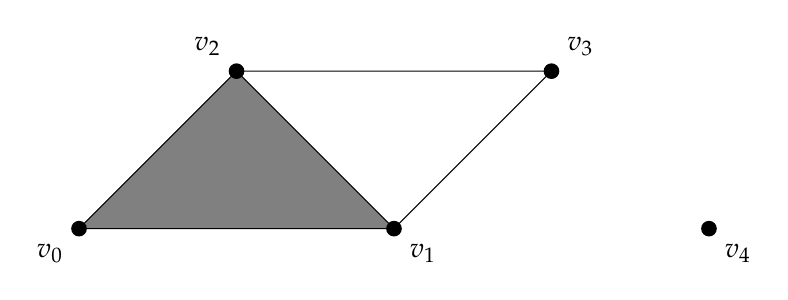
\begin{tikzpicture}

\draw[fill=gray] (0,0) -- (2,2) -- (4,0)-- (0,0);
\draw (2,2) -- (6,2) -- (4,0);

\node[circle, fill=black, inner sep=2pt, label=below left:$v_0 $] (a) at (0,0) {};
\node[circle, fill=black, inner sep=2pt, label=above left:$v_2 $] (b) at (2,2) {};
\node[circle, fill=black, inner sep=2pt, label=below right:$v_1 $] (c) at (4,0) {};
\node[circle, fill=black, inner sep=2pt, label=above right:$v_3 $] (c) at (6,2) {};
\node[circle, fill=black, inner sep=2pt, label=below right:$v_4 $] (c) at (8,0) {};




\end{tikzpicture} \end{center}

One can show that 
\begin{align*}
H_{2}(\mathbf{A}(S/I)) & =\left[\overline{d(v_{1}v_{2}v_{3})}\right]K\\
H_{1}(\mathbf{A}(S/I)) & =\left[\overline{d(v_{1}v_{4})}\right]K.
\end{align*}
In fact, one can show that $H_{i+1}(\mathbf{A}(S/I))\cong\widetilde{H}_{i}(\Delta;K)$,
where $\widetilde{H}_{i}(\Delta;K)$ is the $i$\textbf{th reduced
simplicial homology of $\Delta$ over $K$}. 

\end{example}

\subsection{Hochster's Theorem}

\begin{theorem}\label{theorem} (Hochster) $\beta_{i-1,\sigma}(I_{\Delta})=\beta_{i,\sigma}(S/I_{\Delta})=\text{dim}_{K}\widetilde{H}^{|\sigma|-i-1}(\Delta_{\sigma};K)$
. \end{theorem}

\begin{proof} The first equality is obvious, since a minimal free
resolution of $I_{\Delta}$ is achieved by snipping off the copy of
$S$ occuring in homological degree $0$ of the minimal free resolution
of $S/I_{\Delta}$. For the second equality, we use the commutativity
of $\text{Tor}$: we can calculate $\text{Tor}_{i}^{S}(K,S/I_{\Delta})$
by tensoring the Koszul complex $\mathbb{K}^{\bullet}$ with $S/I_{\Delta}$
as follows.

~~~In each squarefree degree, $(S/I_{\Delta}\otimes_{S}\mathbb{K}^{\bullet})_{\sigma}$
is a quotient of $(\mathbb{K}^{\bullet})_{\sigma}$ and will be the
reduced cochain complex of some simplicial complex. For $\tau\subseteq\sigma$,
the basis vector $e_{\tau\cup\overline{\sigma}}^{\star}=\mathbf{x}^{\tau}\otimes1_{\sigma-\tau}\in(\mathbb{K}^{\bullet})_{\sigma}$
becomes zero in the tensor product $S/I_{\Delta}\otimes\mathbb{K}^{\bullet}$
if and only if $\mathbf{x}^{\tau}=0$ in $S/I_{\Delta}$, and this
occurs if and only if $\tau\notin\Delta$. Therefore, the $K$-basis
for $(S/I_{\Delta}\otimes\mathbb{K}^{\bullet})_{\sigma}$ is $\{e_{\tau\cup\overline{\sigma}}^{\star}\mid\tau\in\Delta_{\sigma}\}$.
Observe that $(S/I_{\Delta}\otimes\mathbb{K}^{\bullet})_{\sigma}\cong\mathcal{C}^{\bullet}(\Delta_{\sigma};K)$,
but considered as a homological complex (decreasing indices) with
$e_{\emptyset}^{\star}$ in homological degree $|\sigma|$, and more
generally $e_{\tau}^{\star}$ in homological degree $|\sigma|-|\tau|=|\sigma|-\text{dim}\tau-1$.
Taking the $i$th homology of this complex yields $\widetilde{H}^{|\sigma|-i-1}(\Delta_{\sigma};K)$
as desired. \end{proof}

\section{$3$-Chain Complexes}

~~~Recall that a chain complex $\mathcal{A}=(A_{\bullet},d_{\bullet})$
is a sequence of $R$-modules $A_{i}$ and morphisms $d_{i}:A_{i}\to A_{i-1}$
\begin{center}\begin{tikzcd} \mathcal{A} := \cdots \arrow[r] & A_{i+1} \arrow[r,"d _{i+1}"] & A_i  \arrow[r," d _i "] & A_{i-1} \arrow[r] & \cdots \end{tikzcd}\end{center}

such that $d_{i}\circ d_{i+1}=0$ for all $i\in\mathbb{Z}$. The condition
$d_{i}\circ d_{i+1}=0$ is equivalent to the condition $\text{Ker}(d_{i})\supset\text{Im}(d_{i+1})$.
With this in mind, we define the $i$th homology of the chain complex
$\mathcal{A}$ to be $H_{i}(\mathcal{A}):=\text{Ker}(d_{i})/\text{Im}(d_{i+1})$.
Chain complexes have been studied quite intensively and are very well
understood. The next definition provides a generalization of a chain
complex:

\begin{defn} A $3$\textbf{-chain complex $\mathcal{A}:=(A_{\bullet},d_{\bullet})$
}is a sequence of $R$-modules $A_{i}$ and morphisms $d_{i}:A_{i}\to A_{i-1}$

\begin{center}\begin{tikzcd} \mathcal{A} := \cdots \arrow[r] & A_{i+1} \arrow[r,"d _{i+1}"] & A_i  \arrow[r," d _i "] & A_{i-1} \arrow[r] & \cdots \end{tikzcd}\end{center}

such that $d_{i-1}\circ d_{i}\circ d_{i+1}=0$ for all $i\in\mathbb{Z}$.
\end{defn}

~~~Since $d_{i}\circ d_{i+1}=0$ implies $d_{i-1}\circ d_{i}\circ d_{i+1}$
for all $i\in\mathbb{Z}$, every chain complex is a $3$-chain complex.
On the other hand, there are interesting examples of $3$-chain complexes
which are not chain complexes, as illustrated in the next proposition. 

\begin{prop}\label{propchaincomplex} Let $I$ be a monomial ideal
in the polynomial ring $\mathbb{F}_{3}[x_{1},\dots,x_{n}]$. For $i\geq0$,
let $A_{i}$ denote the $\mathbb{F}_{3}$-vector space generated by
monomials $x_{1}^{\alpha_{1}}\cdots x_{n}^{\alpha_{n}}$ such that
$\alpha_{1}+\alpha_{2}+\cdots+\alpha_{n}=i$ and $x^{\alpha}\notin I$.
For $i<0$, let $A_{i}=0$. Let $d$ denote the $\mathbb{F}_{3}$-linear
operator $d:=\sum_{k=1}^{n}\partial_{x_{k}}$. Then 

\begin{center}\begin{tikzcd} \mathcal{A} := \cdots \arrow[r] & A_{i+1} \arrow[r,"d _{i+1}"] & A_i  \arrow[r," d _i "] & A_{i-1} \arrow[r] & \cdots \end{tikzcd}\end{center}is
a $3$-chain complex of $\mathbb{F}_{3}$-vector spaces. \end{prop}

\begin{proof} We just need to check that $d^{3}\left(x_{1}^{\alpha_{1}}\cdots x_{n}^{\alpha_{n}}\right)=0$
for any monomial $x_{1}^{\alpha_{1}}\cdots x_{n}^{\alpha_{n}}$ in
$\mathbb{F}_{3}[x_{1},\dots,x_{n}]$. This follows since we are working
mod $3$:
\begin{align*}
d^{3}\left(x_{1}^{\alpha_{1}}\cdots x_{n}^{\alpha_{n}}\right) & =\left(\sum_{k=1}^{n}\partial_{x_{k}}\right)^{3}\left(x_{1}^{\alpha_{1}}\cdots x_{n}^{\alpha_{n}}\right)\\
 & =\left(\sum_{k=1}^{n}\partial_{x_{k}}^{3}\right)\left(x_{1}^{\alpha_{1}}\cdots x_{n}^{\alpha_{n}}\right)\\
 & =\sum_{k=1}^{\infty}\alpha_{k}(\alpha_{k}-1)(\alpha_{k}-2)x_{1}^{\alpha_{k}-2}\\
 & =0.
\end{align*}
\end{proof}

\subsection*{Turning a $3$-Chain Complex into a Chain Complex}

~~~In this section, we desribe how we can obtain a chain complex
from a $3$-complex. Let $\mathcal{A}:=(A_{\bullet},d_{\bullet})$
be a $3$-chain complex. 

\begin{center}\begin{tikzcd} \mathcal{A} := \cdots \arrow[r] & A_{2} \arrow[r,"d_{2}"] &  A_{1} \arrow[r,"d_{1}"] & A_{0} \arrow[r,"d_{0}"] & A_{-1}  \arrow[r," d_{-1} "] & A_{-2} \arrow[r] & \cdots \end{tikzcd}\end{center}

We \textbf{collapse} $\mathcal{A}$ into a chain complex $\mathcal{A}_{\star}$
as follows:

\begin{center}\begin{tikzcd} \mathcal{A_{\star }} := \cdots \arrow[r] A_{5} \arrow[r,"d_4 d_5 "]  & A_{3} \arrow[r,"d_3 "]  & A_{2} \arrow[r,"d_1 d_2 "]  & A_{0} \arrow[r," d_0 "] & A_{-1}  \arrow[r," d_{-2} d _{-1} "] & A_{-3} \arrow[r, "d_{-3}"] & A_{-4} \arrow[r] & \cdots. \end{tikzcd}\end{center}

More formally, $\mathcal{A}_{\star}=(\widetilde{A}_{\bullet},\widetilde{d}_{\bullet})$,
where
\[
\widetilde{A}_{i}=A_{\frac{6i+1+(-1)^{i+1}}{4}}\qquad\widetilde{d}_{i}=\begin{cases}
d_{\frac{6i+1+(-1)^{i+1}}{4}} & \text{if }|i|\text{ is even}\\
d_{\frac{6i-3+(-1)^{i+1}}{4}}d_{\frac{6i+1+(-1)^{i+1}}{4}} & \text{if }|i|\text{ is odd}
\end{cases}
\]

~~~For all $j\in\mathbb{\mathbb{Z}}$, let $\mathcal{A}[j]=(A[j]_{\bullet},d[i]_{\bullet})$
be the sequence of $R$-modules $A[j]_{i}$ are morphisms $d[j]_{i+j}$
where $A[j]_{i}=A_{i+j}$ and $d[j]=d_{i+j}$. It is straightforward
to verify that $\mathcal{A}[j]$ is also a $3$-Chain Complex. We
can also define $\mathcal{A}[1]_{\star}$ and $\mathcal{A}[2]_{\star}$
in a similar way as $\mathcal{A}_{\star}$: 

\begin{center}\begin{tikzcd} 


\mathcal{A}_{\star } := \cdots \arrow[r] A_{5} \arrow[r,"d_4 d_5 "]  & A_{3} \arrow[r,"d_3 "]  & A_{2} \arrow[r,"d_1 d_2 "]  & A_{0} \arrow[r," d_0 "] & A_{-1}  \arrow[r," d_{-2} d _{-1} "] & A_{-3} \arrow[r, "d_{-3}"] & A_{-4} \arrow[r] & \cdots

\\

\mathcal{A}[1]_{\star } := \cdots \arrow[r] A_{6} \arrow[r,"d_5 d_6 "]  & A_{4} \arrow[r,"d_4 "]  & A_{3} \arrow[r,"d_2 d_3 "]  & A_{1} \arrow[r," d_1 "] & A_{0}  \arrow[r," d_{-1} d _{0} "] & A_{-2} \arrow[r, "d_{-2}"] & A_{-3} \arrow[r] & \cdots

\\

\mathcal{A}[2] _{\star } := \cdots \arrow[r] A_{7} \arrow[r,"d_6 d_5 "]  & A_{5} \arrow[r,"d_5 "]  & A_{4} \arrow[r,"d_3 d_4 "]  & A_{2} \arrow[r," d_2 "] & A_{1}  \arrow[r," d_{0} d _{1} "] & A_{-1} \arrow[r, "d_{-1}"] & A_{-2} \arrow[r] & \cdots 


\end{tikzcd}\end{center}

\begin{theorem}\label{theorem} With the notation above, there is
a long exact sequence in homology of the form

\begin{center}\begin{tikzcd}[row sep=30] 

H_{i-1} (\mathcal{A}_{\star } ) \arrow[r]  & \cdots \arrow[d, phantom, ""{coordinate, name=Z}] &  & 

\\

H_i (\mathcal{A}_{\star } ) \arrow[r, "d_{i+1} "]  & H_{i-1} (\mathcal{A}[1]_{\star } ) \arrow[d, phantom, ""{coordinate, name=Z'}] \arrow[r] &  H_{i-2} (\mathcal{A}[2]_{\star } ) \arrow[ull, " d_i ", swap, rounded corners, to path={ -- ([xshift=2ex]\tikztostart.east) |- (Z) [near end]\tikztonodes -| ([xshift=-2ex]\tikztotarget.west) -- (\tikztotarget)}] 

\\

H_{i+1} (\mathcal{A}_{\star } ) \arrow[r]  & H_{i} (\mathcal{A}[1]_{\star } ) \arrow[d, phantom, ""{coordinate, name=Z''}] \arrow[r, "d_{i+2} "] &  H_{i-1} (\mathcal{A}[2]_{\star } ) \arrow[ull, "", swap, rounded corners, to path={ -- ([xshift=2ex]\tikztostart.east) |- (Z') [near end]\tikztonodes -| ([xshift=-2ex]\tikztotarget.west) -- (\tikztotarget)}] 

\\

H_{i+2} (\mathcal{A}_{\star } ) \arrow[r, "d_{i+4} "]  & H_{i+1} (\mathcal{A}[1]_{\star } ) \arrow[d, phantom, ""{coordinate, name=Z'''}] \arrow[r] &  H_i (\mathcal{A}[2]_{\star } ) \arrow[ull, "d_{i+3} ", swap, rounded corners, to path={ -- ([xshift=2ex]\tikztostart.east) |- (Z'') [near end]\tikztonodes -| ([xshift=-2ex]\tikztotarget.west) -- (\tikztotarget)}] 

\\

& \cdots \arrow[r] & H_{i+1} (\mathcal{A}[2]_{\star } ) \arrow[ull, "", swap, rounded corners, to path={ -- ([xshift=2ex]\tikztostart.east) |- (Z''') [near end]\tikztonodes -| ([xshift=-2ex]\tikztotarget.west) -- (\tikztotarget)}] 
 
\end{tikzcd}\end{center}

\end{theorem}

\begin{proof} Let $K_{i}=\text{Ker}(d_{i})/\text{Ker}(d_{i})\cap\text{Im}(d_{i+1})$
for all $i\in\mathbb{Z}$. For each $i\in3\mathbb{Z}$, we have the
following short exact sequences

\begin{center}\begin{tikzcd} 0 \arrow[r] & K_{i+1} \arrow[r]  & H_i (\mathcal{A} _{\star }) \arrow[r, "d_{i+1}"]  & H_{i-1} (\mathcal{A}[1] _{\star })  \arrow[r]  & K_{i} \arrow[r] & 0

\\

0 \arrow[r] & K_{i+2} \arrow[r]  & H_i (\mathcal{A}[1] _{\star }) \arrow[r, "d_{i+2}"]  & H_{i-1} (\mathcal{A}[2] _{\star })  \arrow[r]  & K_{i+1} \arrow[r] & 0

\\

0 \arrow[r] & K_{i+3} \arrow[r]  & H_i (\mathcal{A}[2] _{\star }) \arrow[r, "d_{i+3}"]  & H_{i-1} (\mathcal{A} _{\star })  \arrow[r]  & K_{i+2} \arrow[r] & 0

\end{tikzcd}\end{center}

Connecting these together gives us our desired result. 

\end{proof}

\section{Extra}

\subsection{Measuring The Failure of $\mathbf{A}_{\bullet}(S/I)$ to be a Differential
Graded Algebra over $K$}

~~~In this subsection, we will assume $I$ is just a monomial ideal.
Our task now is to measure the failure of $\mathbf{A}_{\bullet}(S/I)$
to be a differential graded algebra. To do this, we introduce the
following notation. Let $\underline{d}(-,-):(S/I)_{i}\times(S/I)_{j}\to(S/I)_{i+j}$
be the map given by 
\[
\underline{d}(\overline{f},\overline{g})=\underline{d}(\overline{f}\overline{g})+\underline{d}(f)\overline{g}+\overline{f}\underline{d}(\overline{g}).
\]
It is easy to see that bilinearity of $\underline{d}(-,-)$ follows
from bilinearity of multiplication and linearity of $\underline{d}$.
It is also easy to see that $\underline{d}(\overline{f},\overline{g})=0$
if and only if the pair $(\overline{f},\overline{g})\in(S/I)_{i}\times(S/I)_{j}$
satisfies Leibniz law. 

~~~From the bilinearity of $\underline{d}(-,-)$, we see that $\underline{d}(-,-)$
is completely determined by where is maps pairs of monomials $(\overline{m}_{1},\overline{m}_{2})\in(S/I)_{i}\times(S/I)_{j}$. 

\begin{prop}\label{proptrivialleibniz} Suppose $\overline{m}_{1}\overline{m}_{2}\neq0$,
then $\underline{d}(\overline{m}_{1},\overline{m}_{2})=\overline{0}$.
\end{prop}

\begin{proof} Assume $m_{1}$ and $m_{2}$ are already in reduced
form, that is, $m_{1}^{G}=m_{1}$ and $m_{2}^{G}=m_{2}$. Then $m_{1}m_{2}\notin I$
and $m_{1}m_{2}=m_{1}^{G}m_{2}^{G}=(m_{1}m_{2})^{G}$. Therefore
\begin{align*}
\underline{d}(\overline{m}_{1}\overline{m}_{2}) & =\overline{d(m_{1}m_{2})}\\
 & =\overline{d(m_{1})m_{2}+m_{1}d(m_{2})}\\
 & =\overline{d(m_{1})}\overline{m}_{2}+\overline{m}_{1}\overline{d(m_{2})}\\
 & =\underline{d}(\overline{m}_{1})\overline{m}_{2}+\overline{m}_{1}\underline{d}(\overline{m}_{2}).
\end{align*}

\end{proof}

\begin{rem}\label{rem} Actually, $\underline{d}(-,-)$ is completely
determined by where it maps the pairs $(\overline{x}_{\lambda},\overline{m})\in(S/I)_{1}\times(S/I)_{i}$,
where $m$ is a monomial. To see this, suppose $x_{\lambda}\mid m_{1}$
and assume $\underline{d}(\overline{x}_{\lambda},\overline{m})=0$
for every monomial $m$. Then setting $\overline{m}_{1}'=x_{\lambda}^{-1}\overline{m}_{1}$,
and using an inductive argument, we obtain 
\begin{align*}
\underline{d}(\overline{m}_{1}\overline{m}_{2}) & =\underline{d}(x_{\lambda}\overline{m}_{1}'\overline{m}_{2})\\
 & =\overline{m}_{1}'\overline{m}_{2}+\overline{x}_{\lambda}\underline{d}(\overline{m}_{1}'\overline{m}_{2})\\
 & =\overline{m}_{1}'\overline{m}_{2}+\overline{x}_{\lambda}d(\overline{m}_{1}')\overline{m}_{2}+\overline{x}_{\lambda}\overline{m}_{1}'\underline{d}(\overline{m}_{2})\\
 & =\underline{d}(\overline{x}_{\lambda}\overline{m}_{1}')\overline{m}_{2}+\overline{x}_{\lambda}\overline{m}_{1}'\underline{d}(\overline{m}_{2})\\
 & =\underline{d}(\overline{m}_{1})\overline{m}_{2}+\overline{m}_{1}\underline{d}(\overline{m}_{2})
\end{align*}

\end{rem}

\begin{prop}\label{propleibnizequalsboundary} Let $(x_{\lambda},m)\in S_{1}\times S_{i}$
be a pair where $x_{\lambda}$ is not in $I$, $m$ is a monomial
not in $I$, and $x_{\lambda}m$ is in $I$. Then
\[
\underline{d}\left(\overline{x}_{\lambda},\overline{m}\right)=\overline{d(x_{\lambda}m)}.
\]

\end{prop}

\begin{proof} We may assume $x_{\lambda}=x_{\lambda}^{G}$ and $m=m^{G}$,
so that $\underline{d}(\overline{x}_{\lambda})=\overline{d(x_{\lambda})}$
and $\underline{d}(\overline{m})=\overline{d(m)}$. Then
\begin{align*}
\underline{d}\left(\overline{x}_{\lambda},\overline{m}\right) & =\underline{d}(\overline{x_{\lambda}m})+\underline{d}(\overline{x}_{\lambda})\overline{m}+\overline{x}_{\lambda}\underline{d}\left(\overline{m}\right)\\
 & =\underline{d}(\overline{0})+\underline{d}(\overline{x}_{\lambda})\overline{m}+\overline{x}_{\lambda}\underline{d}\left(\overline{m}\right)\\
 & =\underline{d}(\overline{x}_{\lambda})\overline{m}+\overline{x}_{\lambda}\underline{d}\left(\overline{m}\right)\\
 & =\overline{d(x_{\lambda})}\overline{m}+\overline{x}_{\lambda}\overline{d(m)}\\
 & =\overline{d(x_{\lambda}m)}
\end{align*}

\end{proof}
\end{document}
